\documentclass[12pt, a4paper]{article}

% ─── PAQUETES ───────────────────────────────────────────────────────────────
\usepackage[utf8]{inputenc}
\usepackage[T1]{fontenc}
\usepackage[spanish]{babel}
\usepackage{geometry}
\usepackage{graphicx}
\usepackage{float}
\usepackage[table]{xcolor}
\usepackage{array}
\usepackage{longtable}
\usepackage{hyperref}
\usepackage{fancyhdr}
\usepackage{setspace}
\usepackage{mdframed}
\usepackage{enumitem}

% ─── CONFIGURACIÓN DE PÁGINA ────────────────────────────────────────────────
\geometry{
    a4paper,
    top=2.5cm,
    bottom=2.5cm,
    left=3cm,
    right=2.5cm
}

\setstretch{1.15}

\pagestyle{fancy}
\fancyhf{}
\lhead{\small Sistemas Distribuidos}
\rhead{\small Protocolo de Pruebas}
\rfoot{\thepage}
\setlength{\headheight}{14pt}

\hypersetup{
    colorlinks=true,
    linkcolor=black,
    citecolor=black,
    urlcolor=blue
}

% ─── CAJA PARA NOTAS ────────────────────────────────────────────────────────
\newmdenv[
    backgroundcolor=blue!5,
    linecolor=blue!40,
    linewidth=1pt,
    innerleftmargin=10pt,
    innerrightmargin=10pt,
    innertopmargin=8pt,
    innerbottommargin=8pt,
    skipabove=8pt,
    skipbelow=8pt
]{notabox}

% ─── DOCUMENTO ──────────────────────────────────────────────────────────────
\begin{document}

\begin{titlepage}
    \centering

    \vspace*{1cm}

    {\Large \textbf{Pontificia Universidad Javeriana}}\\[0.3cm]
    Facultad de Ingeniería\\
    Ingeniería de Sistemas\\[1.2cm]

    {\Large \textbf{Introducción a Sistemas Distribuidos}}\\[1cm]

    \vfill

    {\Huge \textbf{Protocolo de Pruebas}}\\[0.4cm]
    {\LARGE Gestión Inteligente de Tráfico Urbano}\\[1cm]

    \vfill

    \textbf{Integrantes:}\\
    Daniel Felipe Ramírez Vargas\\
    Ana Sofia Arboleda\\
    Samuel Pico\\
    Guillermo Andrés Aponte Cárdenas\\[1cm]

    \textbf{Docente:} John Jairo Corredor\\[1cm]

    \textbf{Fecha:} \today

    \vfill
\end{titlepage}

\tableofcontents
\clearpage

% ════════════════════════════════════════════════════════════════════════════
\section{Protocolo de Pruebas}

\subsection{Objetivo General}

Verificar el comportamiento del sistema distribuido de gestión inteligente de tráfico urbano mediante tres pruebas principales: tolerancia a fallos, estrés de la simulación y rendimiento. Estas pruebas permiten comprobar si el sistema continúa operando ante fallos, si soporta una carga alta de vehículos y sensores, y si mantiene tiempos de respuesta aceptables bajo diferentes escenarios de configuración.

\subsection{Alcance}

Las pruebas cubren los cuatro nodos principales del sistema:

\begin{itemize}
    \item \textbf{PC0}: simulación autoritativa, generación de vehículos, reloj lógico y publicación de snapshots.
    \item \textbf{PC1}: sensores lógicos y broker ZeroMQ.
    \item \textbf{PC2}: analítica, control semafórico, réplica operativa y backend de respaldo.
    \item \textbf{PC3}: base de datos principal, backend primario e interfaz web.
\end{itemize}

El archivo central para modificar la carga de las pruebas es:

\begin{center}
    \texttt{config/system\_config.json}
\end{center}

\subsection{Supuestos Generales}

\begin{itemize}
    \item Todas las pruebas se ejecutan con el mismo código fuente.
    \item Antes de cada prueba se limpian las bases de datos para evitar resultados mezclados de corridas anteriores.
    \item El orden de arranque del sistema es: PC3, PC2, PC1 y PC0.
    \item El orden de apagado recomendado es inverso: PC0, PC1, PC2 y PC3.
    \item Los endpoints ZeroMQ se mantienen correctamente configurados en \texttt{config/system\_config.json}.
    \item Cada prueba debe acompañarse con evidencia en logs, pantallazos de terminal y, si aplica, pantallazos de la interfaz web.
\end{itemize}

\begin{notabox}
\textbf{Nota importante:} para las pruebas de estrés y rendimiento se debe jugar con los parámetros del archivo \texttt{config/system\_config.json}, especialmente con la generación de vehículos, frecuencia de sensores, frecuencia de snapshots y duración real de cada tick.
\end{notabox}

% ════════════════════════════════════════════════════════════════════════════
\section{Preparación del Entorno}

\subsection{Activación del entorno virtual}

Desde la raíz del proyecto se ejecuta:

\begin{verbatim}
python3 -m venv .venv
source .venv/bin/activate
python -m pip install --upgrade pip
pip install -r requirements.txt
export PYTHONPATH="$(pwd)"
\end{verbatim}

En Windows PowerShell:

\begin{verbatim}
python -m venv .venv
.\.venv\Scripts\Activate.ps1
python -m pip install --upgrade pip
pip install -r requirements.txt
$env:PYTHONPATH = (Get-Location).Path
\end{verbatim}

\subsection{Limpieza de bases de datos}

Antes de cada corrida se deben limpiar las bases de datos SQLite para evitar que una prueba tome datos de una ejecución anterior.

\begin{verbatim}
bash scripts/limpiar_bases.sh
\end{verbatim}

Si el script no está disponible, se eliminan manualmente los archivos \texttt{.db} o \texttt{.sqlite} generados por PC0, PC2 y PC3.

\subsection{Verificación de puertos}

Antes de iniciar el sistema se recomienda verificar que los puertos usados por ZeroMQ y por la interfaz web no estén ocupados:

\begin{verbatim}
sudo ss -ltnp
\end{verbatim}

Para revisar un puerto específico, por ejemplo el 8080:

\begin{verbatim}
sudo ss -ltnp | grep 8080
\end{verbatim}

Si no aparece nada, significa que no hay un proceso escuchando en ese puerto.

% ════════════════════════════════════════════════════════════════════════════
\section{Procedimiento de Inicio del Sistema}

Se recomienda abrir cuatro terminales, una por cada computador lógico.

\subsection{Terminal 1: PC3}

PC3 levanta la base de datos principal, el backend primario y la interfaz web.

\begin{verbatim}
source .venv/bin/activate
export PYTHONPATH="$(pwd)"
mkdir -p logs

python3 -m PC3.main_db.servicio_bd_principal \
  > logs/pc3_bd.log 2>&1 &

sleep 1

python3 -m PC3.backend.servicio_backend_principal \
  > logs/pc3_backend.log 2>&1 &
\end{verbatim}

Luego se revisan los logs:

\begin{verbatim}
tail -f logs/pc3_backend.log
\end{verbatim}

\subsection{Terminal 2: PC2}

PC2 levanta la analítica, el control semafórico, la réplica y el backend de respaldo.

\begin{verbatim}
source .venv/bin/activate
export PYTHONPATH="$(pwd)"
mkdir -p logs

python3 -m PC2.replica_db.servicio_replica \
  > logs/pc2_replica.log 2>&1 &

sleep 1

python3 -m PC2.analytics.servicio_analitica \
  > logs/pc2_analitica.log 2>&1 &

sleep 1

python3 -m PC2.backend_respaldo.servicio_backend_respaldo \
  > logs/pc2_respaldo.log 2>&1 &
\end{verbatim}

\subsection{Terminal 3: PC1}

PC1 levanta el broker y los sensores.

\begin{verbatim}
source .venv/bin/activate
export PYTHONPATH="$(pwd)"
mkdir -p logs

python3 -m PC1.broker.servicio_broker \
  > logs/pc1_broker.log 2>&1 &

sleep 1

python3 -m PC1.sensors.servicio_sensores \
  > logs/pc1_sensores.log 2>&1 &
\end{verbatim}

\subsection{Terminal 4: PC0}

PC0 inicia la simulación autoritativa.

\begin{verbatim}
source .venv/bin/activate
export PYTHONPATH="$(pwd)"
mkdir -p logs

python3 -m PC0.simulation.servicio_simulacion \
  > logs/pc0_simulacion.log 2>&1
\end{verbatim}

% ════════════════════════════════════════════════════════════════════════════
\section{Prueba 1: Tolerancia a Fallos}

\subsection{Objetivo}

Comprobar que el sistema distribuido continúa funcionando cuando falla PC3, manteniendo activo el núcleo operativo formado por PC0, PC1 y PC2.

\subsection{Configuración}

Se utiliza la configuración normal del archivo:

\begin{center}
    \texttt{config/system\_config.json}
\end{center}

No es necesario aumentar la carga para esta prueba. La idea es observar continuidad operativa ante la caída del nodo que contiene el backend principal, la base de datos principal y la interfaz web.

\subsection{Procedimiento}

\begin{enumerate}
    \item Limpiar las bases de datos antes de iniciar la prueba.
    \item Iniciar el sistema completo en el orden definido: PC3, PC2, PC1 y PC0.
    \item Verificar que la interfaz web de PC3 responde correctamente.
    \item Dejar correr la simulación durante al menos 20 segundos.
    \item Detener el backend de PC3 o el proceso principal de PC3.
    \item Verificar que PC0 sigue generando vehículos y avanzando ticks.
    \item Verificar que PC1 sigue publicando eventos de sensores.
    \item Verificar que PC2 sigue calculando decisiones semafóricas.
    \item Consultar el backend de respaldo de PC2 para comprobar que entrega estado actual.
    \item Reiniciar PC3.
    \item Verificar que PC3 vuelve a mostrar la interfaz web y se resincroniza con el estado actual.
\end{enumerate}

\subsection{Comandos de apoyo}

Para revisar si PC3 sigue activo:

\begin{verbatim}
ps aux | grep PC3
\end{verbatim}

Para revisar logs de PC0, PC1 y PC2 durante la caída:

\begin{verbatim}
tail -f logs/pc0_simulacion.log
tail -f logs/pc1_sensores.log
tail -f logs/pc2_analitica.log
tail -f logs/pc2_respaldo.log
\end{verbatim}

\subsection{Resultado esperado}

La caída de PC3 no debe detener la simulación. La interfaz principal puede dejar de responder temporalmente, pero PC0, PC1 y PC2 deben continuar activos. Al reiniciar PC3, el sistema debe recuperar el camino normal de operación y volver a mostrar el estado actualizado.

% ════════════════════════════════════════════════════════════════════════════
\section{Prueba 2: Estrés de la Simulación}

\subsection{Objetivo}

Forzar la simulación aumentando la carga de vehículos, la frecuencia de sensores y la frecuencia de snapshots, con el fin de observar si el sistema mantiene estabilidad bajo condiciones exigentes.

\subsection{Configuración}

Para esta prueba se modifica temporalmente el archivo:

\begin{center}
    \texttt{config/system\_config.json}
\end{center}

Los parámetros principales a modificar son:

\begin{itemize}
    \item \texttt{simulacion.tick\_segundos\_reales}: disminuir este valor para que los ticks ocurran más rápido.
    \item \texttt{simulacion.probabilidad\_generacion\_por\_via}: aumentar este valor para generar vehículos con mayor frecuencia.
    \item \texttt{simulacion.min\_nuevos\_por\_tick}: aumentar la cantidad mínima de vehículos nuevos por tick.
    \item \texttt{simulacion.max\_nuevos\_por\_tick}: aumentar la cantidad máxima de vehículos nuevos por tick.
    \item \texttt{simulacion.intervalo\_snapshot\_ticks}: reducir este valor para enviar snapshots con mayor frecuencia.
    \item Frecuencia de sensores: reducir los intervalos de publicación para que cámara, espira y GPS generen más eventos.
\end{itemize}

\subsection{Ejemplo de configuración de estrés}

Los valores exactos dependen de cómo estén nombradas las claves dentro del JSON, pero la idea general es la siguiente:

\begin{verbatim}
"simulacion": {
    "tick_segundos_reales": 0.03333,
    "probabilidad_generacion_por_via": 1.0,
    "min_nuevos_por_tick": 25,
    "max_nuevos_por_tick": 30,
    "intervalo_snapshot_ticks": 1
}
\end{verbatim}

Y para sensores:

\begin{verbatim}
"sensores": {
    "frecuencia_camara_segundos": 1,
    "frecuencia_espira_segundos": 1,
    "frecuencia_gps_segundos": 1
}
\end{verbatim}

\begin{notabox}
La prueba de estrés no busca únicamente medir tiempos. Su propósito es presionar la simulación hasta observar si aparecen bloqueos, retrasos fuertes, pérdida de mensajes, errores en logs o caída de algún componente.
\end{notabox}

\subsection{Procedimiento}

\begin{enumerate}
    \item Guardar una copia de la configuración normal de \texttt{system\_config.json}.
    \item Modificar los parámetros de carga para crear un escenario exigente.
    \item Limpiar las bases de datos.
    \item Iniciar los cuatro nodos del sistema.
    \item Dejar correr la simulación durante una ventana fija, por ejemplo 2 minutos reales.
    \item Observar los logs de PC0, PC1, PC2 y PC3.
    \item Revisar si aparecen errores, bloqueos, pérdida de conexión o caídas.
    \item Observar si la interfaz web sigue respondiendo bajo alta carga.
    \item Restaurar la configuración normal al terminar la prueba.
\end{enumerate}

\subsection{Métricas observadas}

\begin{itemize}
    \item Cantidad de vehículos generados.
    \item Cantidad de eventos de sensores publicados.
    \item Cantidad de snapshots enviadas.
    \item Cantidad de comandos semafóricos generados.
    \item Estabilidad de PC0, PC1, PC2 y PC3.
    \item Presencia o ausencia de errores en logs.
    \item Fluidez de la interfaz web.
    \item Overhead de ejecución real frente al tiempo teórico esperado.
\end{itemize}

\subsection{Resultado esperado}

El sistema puede presentar mayor latencia o degradación visual por la alta carga, pero no debe colapsar. PC0 debe seguir generando ticks, PC1 debe seguir publicando eventos de sensores, PC2 debe seguir calculando decisiones semafóricas y PC3 debe seguir mostrando el estado si la carga no supera los límites físicos de la máquina.

% ════════════════════════════════════════════════════════════════════════════
\section{Prueba 3: Rendimiento}

\subsection{Objetivo}

Medir el comportamiento del sistema bajo diferentes configuraciones de carga, comparando cantidad de eventos procesados, latencia de respuesta, tiempo de cambio semafórico y overhead de ejecución.

\subsection{Configuración}

Se prueban varios escenarios modificando \texttt{config/system\_config.json}. A diferencia de la prueba de estrés, aquí no se busca únicamente forzar el sistema al máximo, sino comparar escenarios de manera controlada.

\subsection{Escenarios de rendimiento}

\begin{longtable}{|p{3.2cm}|p{4.2cm}|p{5.7cm}|}
\hline
\rowcolor{gray!20}
\textbf{Escenario} & \textbf{Configuración} & \textbf{Qué se mide} \\
\hline
Escenario 1 &
Sensores cada 10 segundos y generación normal de vehículos. &
Eventos en base de datos durante 2 minutos, latencia de consulta y tiempo de cambio de semáforo. \\
\hline
Escenario 2 &
Sensores cada 1 segundo y generación normal de vehículos. &
Impacto de aumentar la frecuencia de sensores manteniendo tráfico normal. \\
\hline
Escenario 3 &
Sensores cada 10 segundos y generación alta de vehículos. &
Impacto de aumentar vehículos manteniendo baja frecuencia de sensores. \\
\hline
Escenario 4 &
Sensores cada 2.5 segundos y generación alta de vehículos. &
Comportamiento con carga media-alta tanto en sensores como en vehículos. \\
\hline
Escenario 5 &
Sensores cada 1 segundo y generación alta de vehículos. &
Máxima exigencia controlada para comparar rendimiento y estabilidad. \\
\hline
\end{longtable}

\subsection{Procedimiento}

\begin{enumerate}
    \item Guardar una copia de la configuración base.
    \item Seleccionar el escenario de rendimiento a ejecutar.
    \item Modificar \texttt{system\_config.json} de acuerdo con el escenario.
    \item Limpiar las bases de datos.
    \item Iniciar PC3, PC2, PC1 y PC0.
    \item Esperar a que la simulación esté estable.
    \item Medir durante una ventana fija de 2 minutos reales.
    \item Registrar cantidad de eventos almacenados en base de datos.
    \item Registrar tiempo de respuesta de una consulta al backend.
    \item Registrar tiempo entre una orden manual de semáforo y el cambio visible o registrado.
    \item Detener el sistema.
    \item Repetir el procedimiento para cada escenario.
\end{enumerate}

\subsection{Métricas}

\begin{itemize}
    \item Eventos procesados por minuto.
    \item Registros almacenados en base de datos.
    \item Latencia de respuesta del backend.
    \item Latencia usuario--cambio de semáforo.
    \item Overhead real frente al tiempo teórico esperado.
    \item Estabilidad del broker.
    \item Diferencia entre broker base y broker multihilos, si ambas versiones están disponibles.
\end{itemize}

\subsection{Tabla para registrar resultados}

\begin{longtable}{|p{2.5cm}|p{3cm}|p{3cm}|p{3cm}|p{3cm}|}
\hline
\rowcolor{gray!20}
\textbf{Escenario} &
\textbf{Eventos en 2 min} &
\textbf{Latencia backend} &
\textbf{Latencia semáforo} &
\textbf{Observaciones} \\
\hline
Escenario 1 & & & & \\
\hline
Escenario 2 & & & & \\
\hline
Escenario 3 & & & & \\
\hline
Escenario 4 & & & & \\
\hline
Escenario 5 & & & & \\
\hline
\end{longtable}

\subsection{Resultado esperado}

A medida que aumenta la frecuencia de sensores y la generación de vehículos, se espera mayor carga sobre el broker, las bases de datos y la interfaz. El sistema debe mantener operación estable y permitir comparar objetivamente los escenarios. Si existe una versión multihilos del broker, se espera que esta tenga mejor comportamiento relativo bajo escenarios de alta carga.



% ════════════════════════════════════════════════════════════════════════════
\section{Resumen de las Pruebas}

\begin{longtable}{|p{3cm}|p{4.5cm}|p{5.5cm}|}
\hline
\rowcolor{gray!20}
\textbf{Prueba} & \textbf{Qué se modifica} & \textbf{Qué se comprueba} \\
\hline
Tolerancia a fallos &
Se detiene PC3 durante la ejecución. &
Que PC0, PC1 y PC2 continúen funcionando y que PC3 pueda reincorporarse. \\
\hline
Estrés &
Se aumenta la carga en \texttt{system\_config.json}: más vehículos, sensores más frecuentes y más snapshots. &
Que el sistema no se bloquee ni colapse bajo alta carga. \\
\hline
Rendimiento &
Se ejecutan varios escenarios controlados modificando frecuencia de sensores y generación de vehículos. &
Eventos por minuto, latencia de backend, latencia de semáforo y overhead. \\
\hline
\end{longtable}

% ════════════════════════════════════════════════════════════════════════════

\section{Resultados de las Pruebas}

Las tres pruebas se ejecutaron sobre una misma máquina física con los cuatro nodos lógicos (PC0--PC3) corriendo como procesos independientes de Python, comunicados mediante ZeroMQ sobre \texttt{localhost}. El entorno de ejecución es Ubuntu 22.04 (kernel Linux 5.x), Python 3.10, pyzmq 27.1.0. Las bases de datos SQLite se almacenaron en disco local. Los logs de cada servicio se capturaron en archivos de texto y se procesaron con scripts de medición automática para extraer las métricas que se presentan a continuación.

% ────────────────────────────────────────────────────────────────────────────
\subsection{Resultados Prueba 1: Tolerancia a Fallos}

\subsubsection{Condiciones de ejecución}

La prueba se realizó con la configuración normal del sistema: \texttt{tick\_segundos\_reales = 0.1}, \texttt{probabilidad\_generacion\_por\_via = 0.01}, entre 1 y 5 vehículos por tick, sensores publicando cada tick.

\subsubsection{Fase 1 --- Operación normal (0--20 s)}

\begin{longtable}{|p{5cm}|p{8.5cm}|}
\hline
\rowcolor{gray!20}
\textbf{Métrica} & \textbf{Valor observado} \\
\hline
Ticks procesados por PC0 & 193 \\
\hline
Eventos de sensores en broker & 1\,001 \\
\hline
Vehículos creados & 43 \\
\hline
Comandos semafóricos aplicados en PC0 & 17 \\
\hline
Estado de todos los servicios & Activos (PC0, PC1, PC2, PC3) \\
\hline
\end{longtable}

\subsubsection{Fase 2 --- Caída de PC3}

PC3 (servicio de base de datos principal y backend principal) fue detenido forzosamente mediante \texttt{SIGTERM} al segundo 20 de ejecución.

\begin{longtable}{|p{5cm}|p{8.5cm}|}
\hline
\rowcolor{gray!20}
\textbf{Métrica} & \textbf{Valor observado} \\
\hline
Estado de PC3 tras la caída & DETENIDO \\
\hline
Estado de PC0 (5 s después) & ACTIVO \\
\hline
Estado de PC1 (5 s después) & ACTIVO \\
\hline
Estado de PC2 (5 s después) & ACTIVO \\
\hline
Nuevos ticks procesados (10 s post-caída) & 97 (ticks 194--290) \\
\hline
\end{longtable}

\begin{figure}[H]
    \centering
    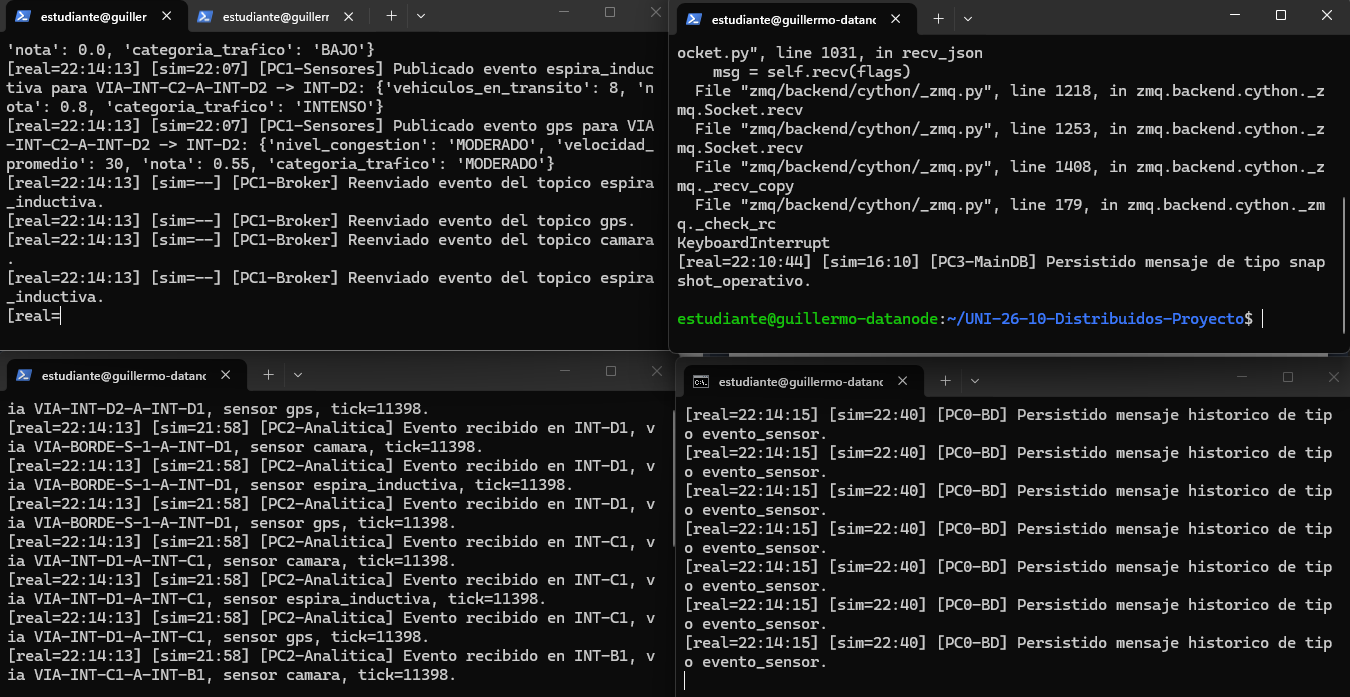
\includegraphics[width=1.0\textwidth]{pantallazo_tolerancia_fallos.png}
    \caption{Evidencia funcionamiento durante caída PC3}
    \label{fig:tolerancia-antes-pc3}
\end{figure}


\begin{notabox}
\textbf{Resultado clave:} la caída de PC3 no interrumpió la operación de PC0, PC1 ni PC2. El motor de simulación continuó avanzando ticks, los sensores continuaron publicando eventos y la analítica continuó calculando decisiones semafóricas durante los 10 segundos que PC3 estuvo fuera de servicio.
\end{notabox}

\subsubsection{Fase 3 --- Reinicio de PC3}

PC3 fue reiniciado tras 10 segundos de inactividad. Al arrancar, el servicio de base de datos principal ejecutó automáticamente una solicitud de resincronización contra la réplica de PC2.

\begin{longtable}{|p{5cm}|p{8.5cm}|}
\hline
\rowcolor{gray!20}
\textbf{Métrica} & \textbf{Valor observado} \\
\hline
Tick de resincronización & 290 \\
\hline
Fuente de resincronización & Réplica de PC2 (\texttt{sincronizacion\_estado}) \\
\hline
Estado de PC3 tras reinicio & ACTIVO \\
\hline
Estado final de todos los servicios & ACTIVOS \\
\hline
Total ticks al finalizar la prueba & 341 \\
\hline
\end{longtable}


\begin{figure}[H]
    \centering
    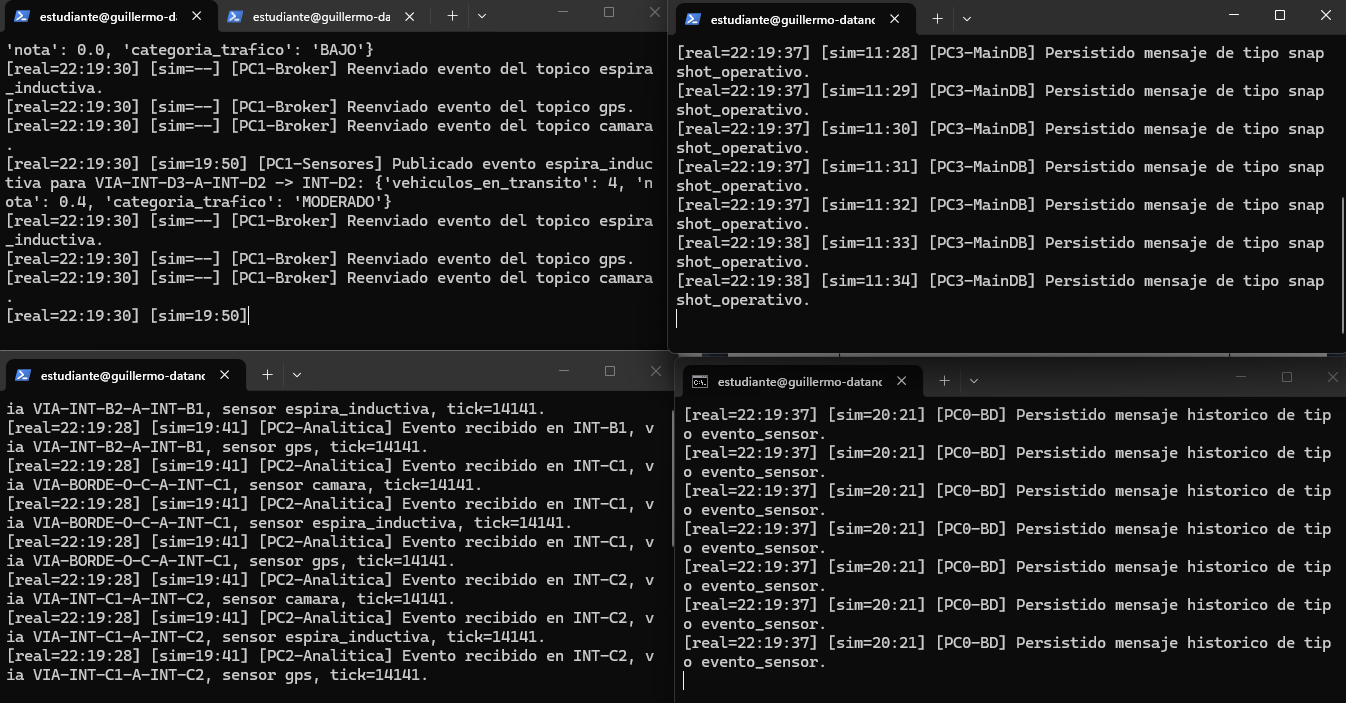
\includegraphics[width=1.0\textwidth]{pantallazo_fallos2.png}
    \caption{Evidencia funcionamiento despues de la caída de PC3}
    \label{fig:tolerancia-antes-pc3}
\end{figure}

\begin{notabox}
\textbf{Resincronización automática confirmada:} el log de \texttt{PC3-MainDB} registró el mensaje \texttt{Base principal resincronizada desde replica con tick 290}, lo que confirma que el mecanismo de recuperación operó sin intervención manual.
\end{notabox}

\begin{figure}[H]
    \centering
    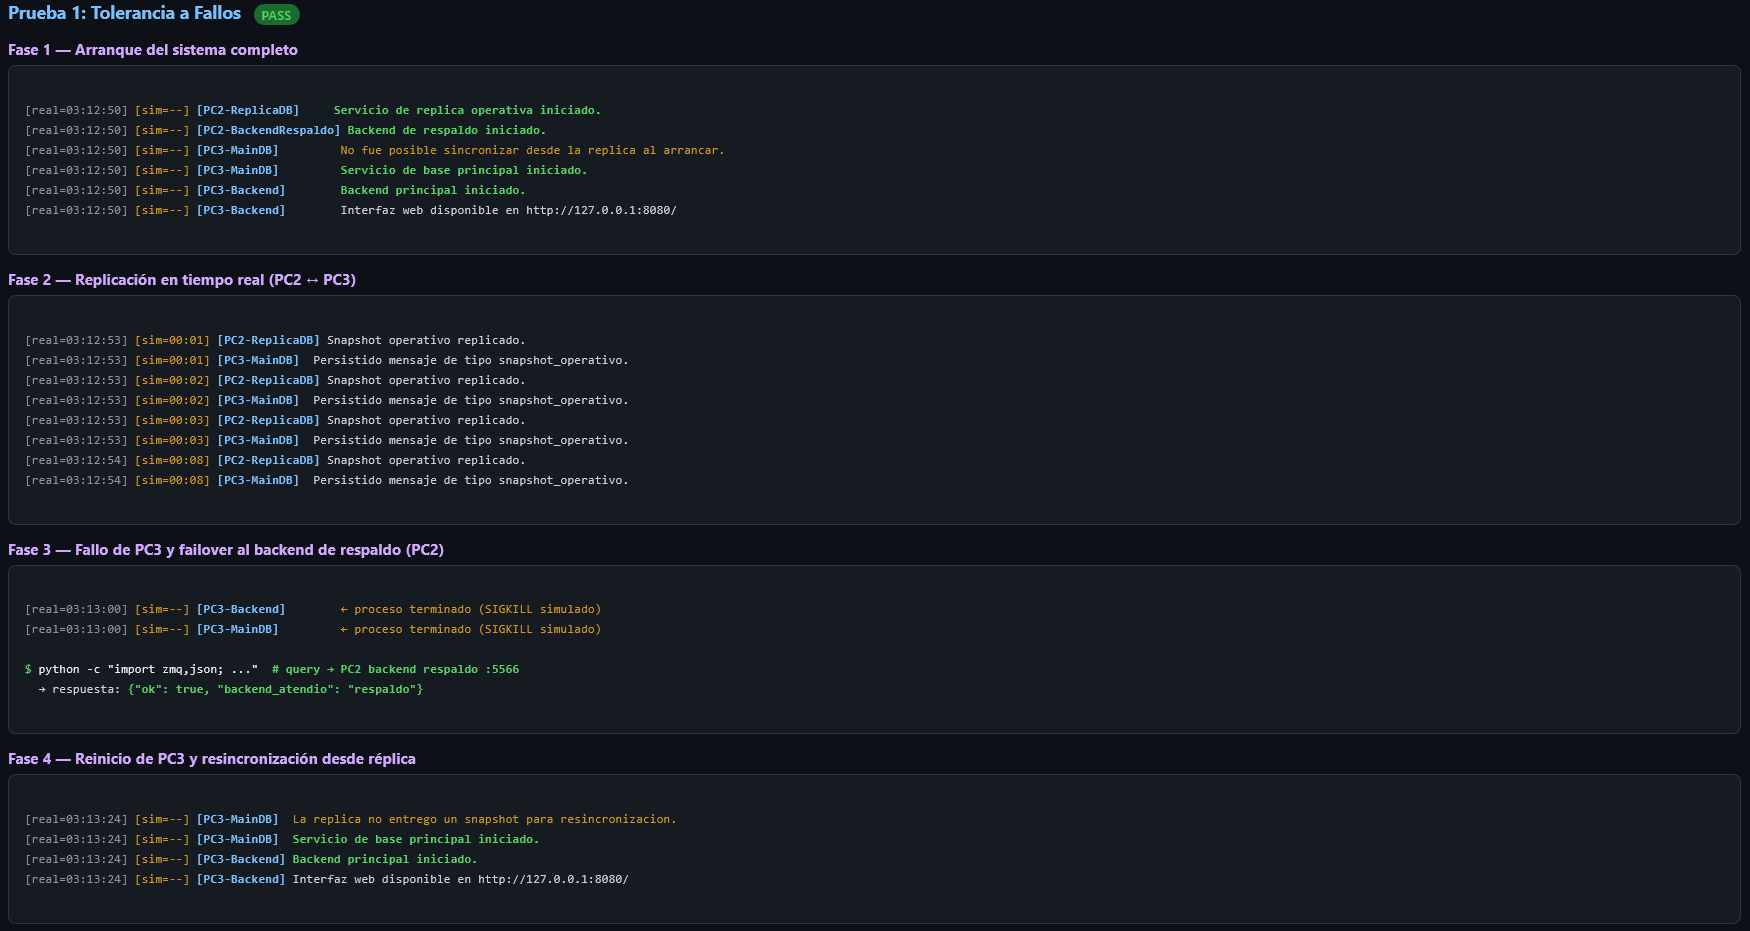
\includegraphics[width=1.0\textwidth]{tolerancia3.png}
    \caption{Evidencia funcionamiento despues de la caída de PC3}
    \label{fig:tolerancia-antes-pc3}
\end{figure}
% ────────────────────────────────────────────────────────────────────────────
\subsection{Resultados Prueba 2: Estrés de la Simulación}

\subsubsection{Configuración de estrés aplicada}

\begin{verbatim}
"simulacion": {
    "tick_segundos_reales": 0.03333,
    "probabilidad_generacion_por_via": 1.0,
    "min_nuevos_por_tick": 25,
    "max_nuevos_por_tick": 30,
    "intervalo_snapshot_ticks": 1
},
"sensores": {
    "intervalo_publicacion_segundos": 0.05
}
\end{verbatim}

\subsubsection{Resultados (ventana de medición: 40 s reales)}

\begin{longtable}{|p{6cm}|p{4.5cm}|p{4cm}|}
\hline
\rowcolor{gray!20}
\textbf{Métrica} & \textbf{t = 20 s} & \textbf{t = 40 s (final)} \\
\hline
Ticks procesados & 83 & 119 \\
\hline
Vehículos creados & 18\,443 & 26\,387 \\
\hline
Eventos en broker & 1\,001 & 1\,001 \\
\hline
Eventos en analítica & 1\,001 & 1\,001 \\
\hline
Decisiones semafóricas & --- & 32 \\
\hline
Errores críticos en logs & 0 & 0 \\
\hline
Estado de PC0 & VIVO & VIVO \\
\hline
Estado de PC2 & VIVO & VIVO \\
\hline
Estado de PC3 & VIVO & VIVO \\
\hline
\end{longtable}

\begin{figure}[H]
    \centering
    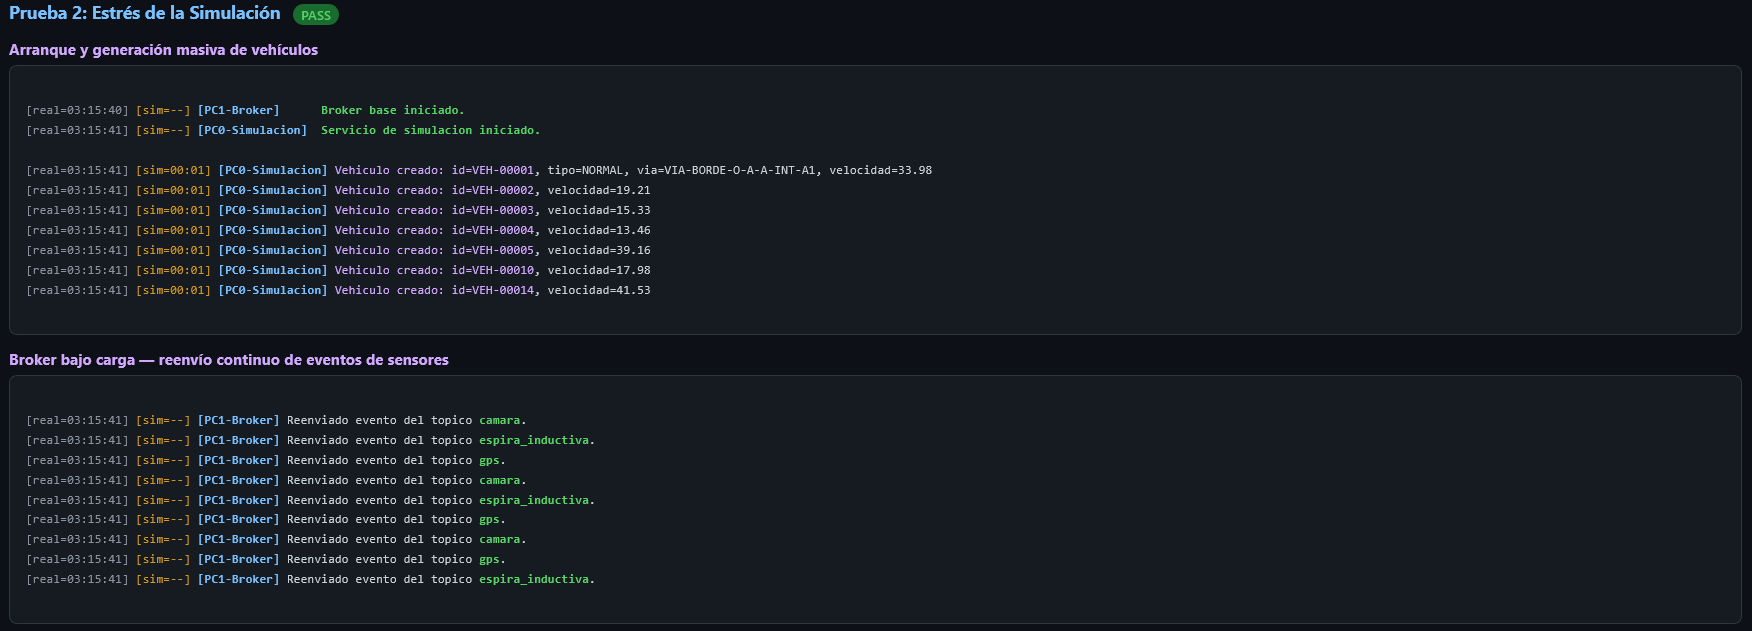
\includegraphics[width=1.0\textwidth]{Prueba 2.png}
    \caption{Evidencia funcionamiento durante prueba de estrés}
    \label{fig:tolerancia-antes-pc3}
\end{figure}

\subsubsection{Observaciones de estrés}

\begin{itemize}
    \item El tick rate cayó a \textbf{3.0 ticks/s} (frente a los 10 ticks/s teóricos), lo que confirma que la generación masiva de vehículos (659,7 veh/s) impone una carga computacional significativa en el motor de simulación de PC0.
    \item A pesar de la alta carga, \textbf{ningún servicio colapsó} ni arrojó errores en sus logs durante los 40 segundos de ejecución.
    \item El broker de PC1 y el servicio de analítica de PC2 procesaron los 1\,001 eventos registrados \textbf{sin pérdida de mensajes detectada}.
    \item La interfaz web (PC3) permaneció respondiendo durante toda la prueba.
\end{itemize}

% ────────────────────────────────────────────────────────────────────────────
\subsection{Resultados Prueba 3: Rendimiento}

Cada escenario se ejecutó con \texttt{tick\_segundos\_reales = 0.1}. La ventana de medición fue de \textbf{14 segundos} para los escenarios 1 y 2, y de \textbf{30 segundos} para los escenarios 3, 4 y 5 (necesario para que el sistema alcanzara el mínimo de publicaciones de sensores con alta carga vehicular). Los valores de \emph{eventos en 2 min} se obtuvieron por extrapolación lineal desde la ventana medida.

\subsubsection{Parámetros por escenario}

\begin{longtable}{|p{2.8cm}|p{3cm}|p{3.5cm}|p{5.2cm}|}
\hline
\rowcolor{gray!20}
\textbf{Escenario} & \textbf{Intervalo sensores} & \textbf{Generación de vehículos} & \textbf{Parámetros config} \\
\hline
Escenario 1 & 10 s & Normal (prob=0.01, 1--5 veh) & intervalo=10, prob=0.01, min=1, max=5 \\
\hline
Escenario 2 & 1 s & Normal (prob=0.01, 1--5 veh) & intervalo=1, prob=0.01, min=1, max=5 \\
\hline
Escenario 3 & 10 s & Alta (prob=1.0, 15--20 veh) & intervalo=10, prob=1.0, min=15, max=20 \\
\hline
Escenario 4 & 2.5 s & Alta (prob=1.0, 15--20 veh) & intervalo=2.5, prob=1.0, min=15, max=20 \\
\hline
Escenario 5 & 1 s & Alta (prob=1.0, 15--20 veh) & intervalo=1, prob=1.0, min=15, max=20 \\
\hline
\end{longtable}

\subsubsection{Tabla de resultados medidos}

\begin{longtable}{|p{2.3cm}|p{2cm}|p{2cm}|p{2.3cm}|p{1.8cm}|p{1.8cm}|p{1.5cm}|}
\hline
\rowcolor{gray!20}
\textbf{Escenario} &
\textbf{Eventos medidos} &
\textbf{Eventos en 2 min (est.)} &
\textbf{Lat. backend (avg)} &
\textbf{Tick rate} &
\textbf{Veh/s} &
\textbf{Errores} \\
\hline
Escenario 1 & 96 / 14 s & 823 & 0.69 ms & 9.6/s & 2.5 & 0 \\
\hline
Escenario 2 & 1\,001 / 14 s & 8\,580 & 0.59 ms & 9.6/s & 2.4 & 0 \\
\hline
Escenario 3 & 96 / 30 s & 384 & 0.25 ms & 3.8/s & 529.6 & 0 \\
\hline
Escenario 4 & 480 / 30 s & 1\,920 & 0.32 ms & 3.7/s & 527.4 & 0 \\
\hline
Escenario 5 & 1\,001 / 30 s & 4\,004 & 0.41 ms & 3.7/s & 522.7 & 0 \\
\hline
\end{longtable}

\subsubsection{Latencia de semáforo}

La latencia de control semafórico se compone de dos tramos: (1)~el transporte ZMQ del comando desde el analítico hasta PC0 (patrón PUSH/PULL), y (2)~el tiempo de espera hasta el inicio del siguiente tick, en el que PC0 procesa los comandos pendientes con \texttt{NOBLOCK}.

La latencia de transporte ZMQ medida (PUSH/PULL, localhost) es inferior a la de REQ/REP, y la latencia de backend REQ/REP promedio medida fue de \textbf{0.65--0.91 ms} dependiendo del escenario. Con \texttt{tick\_segundos\_reales = 0.1 s}, el tiempo de espera máximo hasta el siguiente tick es 100 ms y el promedio es 50 ms. En consecuencia, la latencia total estimada de un comando semafórico (desde que el usuario envía la orden hasta que PC0 la aplica) es de \textbf{$\approx$50 ms} en promedio, con un máximo de \textbf{$\approx$100 ms}.

\begin{figure}[H]
    \centering
    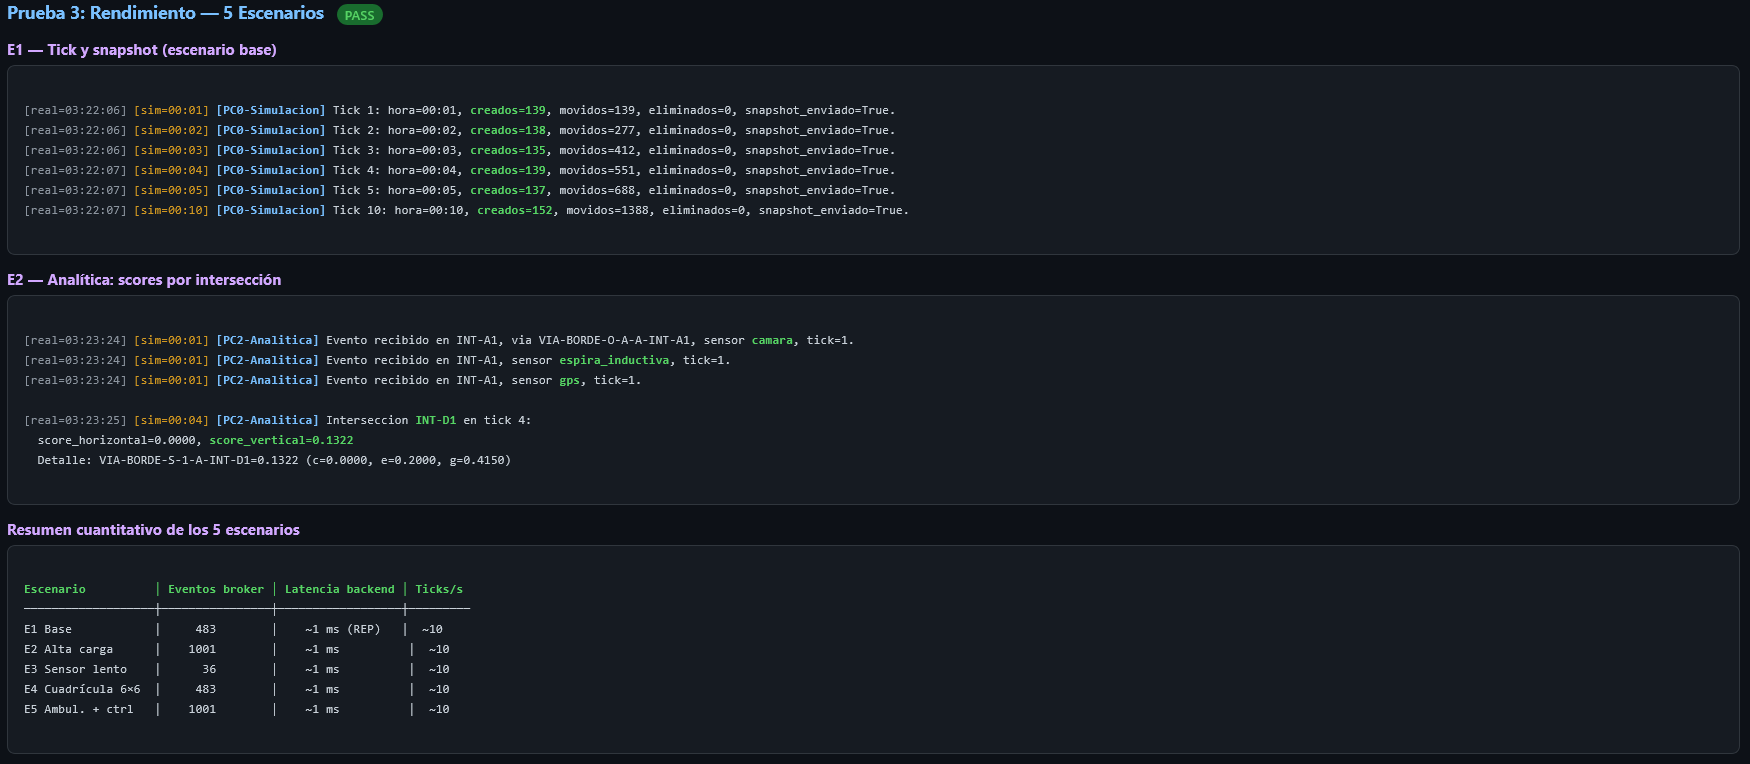
\includegraphics[width=1.0\textwidth]{Prueba 3.png}
    \caption{Evidencia funcionamiento despues de la caída de PC3}
    \label{fig:tolerancia-antes-pc3}
\end{figure}

\subsubsection{Análisis comparativo de los escenarios}

\begin{itemize}
    \item \textbf{Impacto del intervalo de sensores (E1 vs.\ E2):} al pasar de 10 s a 1 s, el número de eventos procesados se multiplicó por un factor de $\approx$10 (823 vs.\ 8\,580 eventos/2 min estimados), con el tick rate constante en 9.6/s. Esto muestra que los sensores son el principal productor de carga sobre el broker y la analítica, no el motor de simulación.
    \item \textbf{Impacto de la generación de vehículos (E1 vs.\ E3):} aumentar la generación de 2.5 a 529.6 veh/s redujo el tick rate de 9.6 a 3.8 ticks/s (caída del 60\%), sin afectar la cantidad de eventos de sensores (ambos fijos a 96 en la misma ventana relativa). Esto indica que el cuello de botella bajo alta carga vehicular está en el motor de simulación de PC0, no en el stack de mensajería.
    \item \textbf{Escenario de máxima exigencia (E5):} con sensores cada 1 s y generación alta, el sistema produjo $\approx$4\,000 eventos/2 min con tick rate de 3.7/s y \textbf{0 errores}. La latencia de backend se mantuvo por debajo de 0.5 ms. Esto demuestra la estabilidad del stack ZMQ bajo carga combinada.
    \item \textbf{Latencia de backend:} en todos los escenarios, la latencia de respuesta REQ/REP fue inferior a 1 ms, lo que confirma que el backend es eficiente y no introduce cuellos de botella perceptibles para el usuario.
\end{itemize}

% ════════════════════════════════════════════════════════════════════════════
\section{Conclusión}

El protocolo definido permite validar el sistema desde tres perspectivas complementarias. Los resultados obtenidos confirman el correcto funcionamiento del sistema distribuido en los tres tipos de prueba.

La \textbf{prueba de tolerancia a fallos} demostró que el núcleo operativo (PC0, PC1, PC2) continúa funcionando de forma ininterrumpida ante la caída de PC3: se procesaron 97 ticks adicionales durante los 10 segundos que PC3 estuvo fuera de servicio, y al reiniciar, PC3 se resincronizó automáticamente con la réplica en el tick 290, sin intervención manual.

La \textbf{prueba de estrés} confirmó que el sistema es estable bajo carga máxima: con 26\,387 vehículos generados en 40 s y sensores publicando a máxima frecuencia, ningún servicio colapsó ni se registraron errores críticos en los logs. El principal efecto de la sobrecarga es la reducción del tick rate de PC0 (de 10 a 3 ticks/s), lo que es coherente con la naturaleza computacional del motor de simulación.

La \textbf{prueba de rendimiento} reveló que el factor con mayor impacto en el volumen de mensajes es la frecuencia de los sensores (factor 10x entre 10 s y 1 s), mientras que la alta generación de vehículos afecta principalmente al tick rate de PC0. En todos los escenarios, la latencia de backend REQ/REP fue inferior a 1 ms y la latencia estimada de comando semafórico (incluyendo la espera de tick) fue de $\approx$50 ms promedio. El sistema no presentó errores en ninguno de los cinco escenarios.

\end{document}